\documentclass[conference]{IEEEtran}

% --- Encoding / fuentes ---
\usepackage[utf8]{inputenc}
\usepackage[T1]{fontenc}

% --- Utilidades básicas ---
\usepackage{graphicx}
\usepackage{amsmath, amssymb}
\usepackage{url}
\usepackage{microtype} % opcional, recomendado
\usepackage{subfig}
% Requiere en el preámbulo:
% \usepackage{subfig}
\usepackage{tikz}
\usetikzlibrary{positioning,arrows.meta,calc}

% --- TikZ (pipeline) + TikZ-CD (diagramas conmutativos) ---
\usepackage{tikz}
\usetikzlibrary{arrows.meta,positioning,shapes.geometric,calc}
\usepackage{tikz-cd}
\usepackage{adjustbox}
\usepackage{float}    
\usepackage{placeins}  
\usepackage{fancyhdr}
\pagestyle{fancy}
\fancyhf{}
\fancyfoot[C]{\thepage}
\renewcommand{\headrulewidth}{0pt}
\renewcommand{\footrulewidth}{0pt}

\title{Segmentación automática de columna vertebral y vértebras en radiografías con escoliosis para entornos con recursos computacionales limitados}

\author{
\IEEEauthorblockN{Jason Rosher Morrill, John Williams Morrill, David Alan Delgado Zarco, Octavio Esquivel Álvarez del Castillo}
\IEEEauthorblockA{Maestría en Inteligencia Artificial (MAIA)\\
Universidad de los Andes, Bogotá, Colombia\\
j.morrill@uniandes.edu.co, j.williams@uniandes.edu.co, d.delgado@uniandes.edu.co, o.esquivel@uniandes.edu.co}
}

\begin{document}
\maketitle
\thispagestyle{fancy}

\begin{abstract}

La segmentación automática de la columna vertebral en radiografías 2D es una tarea compleja debido a la superposición de estructuras anatómicas, la variabilidad morfológica entre pacientes, el ruido radiográfico y la limitada disponibilidad de datos clínicos anotados. En este trabajo se propone un enfoque híbrido para la segmentación y caracterización geométrica de la columna vertebral en radiografías con escoliosis, combinando redes neuronales convolucionales, canales geométricos derivados de la curva vertebral, análisis frecuencial de gaps y picos intervertebrales, análisis topológico de datos (TDA) y clusterización regional. La columna se modela como una secuencia ordenada de parches anatómicos indexados sobre una curva central, lo que permite preservar relaciones espaciales entre regiones consecutivas. La CNN multicanal y multisalida integra información de intensidad radiográfica, bandas anatómicas, bordes, respuestas orientadas y descriptores geométricos locales para producir máscaras binarias, segmentación regional, mapas de borde, espacios intervertebrales y representaciones ordinales. Posteriormente, las salidas del modelo se reorganizan anatómicamente para construir vectores regionales utilizados en clustering y TDA. Los resultados preliminares muestran que la representación propuesta captura información estructural relevante de la columna vertebral y permite generar agrupamientos regionales asociados con patrones normales y escolióticos. En conjunto, este trabajo plantea que la segmentación vertebral puede entenderse no solo como una tarea de predicción píxel a píxel, sino como la construcción de una representación anatómica, geométrica y topológica útil para el análisis computacional de la escoliosis.

\end{abstract}

\begin{IEEEkeywords}
spine segmentation, scoliosis, convolutional neural networks, anatomical curve, geometric channels, vertebral patches, intervertebral gaps, frequency analysis, regional clustering, topological data analysis
\end{IEEEkeywords}

\section{Introducción}

La escoliosis es una deformidad tridimensional de la columna vertebral caracterizada por una curvatura lateral anormal acompañada de rotación vertebral. Esta condición puede progresar durante el crecimiento y afectar significativamente la postura, la función respiratoria y la calidad de vida de los pacientes. El diagnóstico y seguimiento clínico se realizan principalmente mediante radiografías anteroposteriores de columna vertebral.

La severidad de la escoliosis se evalúa clínicamente mediante el ángulo de Cobb, el cual se calcula identificando manualmente las vértebras límite de la curvatura y midiendo el ángulo formado entre sus placas terminales. Aunque este método es ampliamente utilizado en la práctica clínica, su estimación depende de la selección manual de puntos anatómicos, lo que introduce variabilidad entre observadores y reduce la reproducibilidad de las mediciones.

Los avances recientes en aprendizaje profundo han permitido desarrollar métodos automáticos para el análisis de imágenes médicas, incluyendo la segmentación de estructuras anatómicas y la estimación de métricas clínicas. Sin embargo, muchos enfoques se basan únicamente en representaciones locales aprendidas por redes convolucionales, sin incorporar explícitamente información geométrica o topológica de la estructura de la columna vertebral.

En este trabajo se propone un enfoque híbrido que combina redes convolucionales, análisis topológico de datos y la geometría de la columna vertebral a partir de radiografías. La idea central consiste en enriquecer las representaciones obtenidas por redes convolucionales con información estructural derivada de la segmentación vertebral, permitiendo estimar automáticamente métricas clínicas como el ángulo de Cobb y caracterizar la deformidad espinal.

Las principales contribuciones de este trabajo son:

\begin{itemize}

\item Un pipeline computacional para el análisis automático de radiografías de columna vertebral.

\item La integración de representaciones geométricas y topológicas derivadas de la segmentación vertebral.

\item Un marco experimental escalable para la ejecución paralela de experimentos y evaluación de modelos.

\item La estimación automática de métricas clínicas relevantes para la evaluación de la escoliosis.

\end{itemize}

\section{Objetivos}

\subsection{Objetivo general}

Desarrollar un modelo híbrido basado en CNN, análisis topológico de datos y Transformers kernelizados para la segmentación automática de vértebras y la estimación del ángulo de Cobb en radiografías de columna vertebral.

\subsection{Objetivos específicos}

\begin{itemize}

\item Diseñar una arquitectura que combine representaciones convolucionales, topológicas y geométricas.

\item Implementar un Transformer multi-kernel capaz de integrar múltiples espacios de representación.

\item Evaluar el desempeño del modelo en tareas de segmentación vertebral utilizando métricas estándar de segmentación médica.

\item Analizar el impacto de descriptores topológicos en la coherencia anatómica de la segmentación.

\end{itemize}

\section{Estado del Arte}
\label{sec:sota}
La segmentación automática de columna y vértebras ha avanzado de manera importante con el uso de arquitecturas profundas, especialmente modelos tipo U-Net y sus variantes. Estos enfoques han demostrado ser efectivos en segmentación médica al combinar extracción local de rasgos con una estructura encoder--decoder capaz de recuperar información espacial. En estudios de tomografía computarizada 3D, métodos como U-Net y nnU-Net han servido como referencias sólidas para la segmentación vertebral multi-etiqueta \cite{ronneberger2015unet,isensee2021nnunet}.

Más recientemente, se han incorporado modelos basados en Transformers para capturar relaciones de largo alcance y mejorar la consistencia anatómica de las predicciones. Estos métodos han sido útiles en escenarios donde el campo de visión varía y el número de vértebras visibles no es constante \cite{tao2022spine_transformers,you2023verteformer,zhang2023swinspine,li2024verformer}. Algunas propuestas emplean mecanismos de atención para representar vértebras como instancias anatómicas, mientras que otras integran módulos Transformer dentro de arquitecturas tipo U-Net para complementar las convoluciones con información contextual global \cite{you2022eg_trans3dunet,you2023verteformer,zhang2023swinspine}.

A pesar de estos avances, la segmentación vertebral en radiografías 2D continúa siendo un problema desafiante. A diferencia de la tomografía, las radiografías presentan superposición de estructuras, variabilidad de contraste, ruido y deformaciones anatómicas asociadas con la escoliosis. Además, muchos métodos se enfocan principalmente en la segmentación píxel a píxel y utilizan información geométrica de manera limitada, por ejemplo mediante centroides, bordes, cajas o mapas auxiliares \cite{you2022eg_trans3dunet,aydogdu2024centroid,li2024verformer}.

En este contexto, existe una oportunidad para explorar representaciones anatómicas más estructuradas, donde la columna no se modele únicamente como una máscara, sino como una curva organizada con regiones locales, relaciones espaciales y descriptores geométricos. De manera complementaria, herramientas como el análisis topológico de datos pueden aportar información sobre conectividad, forma y organización global de las estructuras segmentadas \cite{clough2020topological,hu2019topology}. Por ello, este trabajo se orienta a combinar CNN, canales geométricos, curva anatómica, análisis de gaps intervertebrales y clusterización regional como una alternativa para enriquecer la representación de la columna vertebral en radiografías con escoliosis.



\section{Marco Teórico}
\subsection{Imágenes médicas como espacios discretos}
Una imagen médica digital puede representarse como una función definida sobre una rejilla discreta de píxeles. En el caso de una radiografía, cada píxel contiene información de intensidad asociada a la absorción de rayos X en una región anatómica específica.
Matemáticamente, una imagen puede modelarse como:

\[
I:\Omega \subset \mathbb{Z}^2 \rightarrow \mathbb{R}
\]

donde $\Omega$ representa el dominio discreto de la imagen e $I(x,y)$ representa la intensidad del píxel ubicado en la coordenada $(x,y)$.

Esta representación permite analizar la imagen no solamente como una matriz numérica, sino también como un espacio discreto con estructura espacial, vecindades, regiones conectadas y subconjuntos anatómicos de interés.

\subsection{Espacios topológicos discretos}

Un espacio topológico es un conjunto $X$ junto con una colección $\mathcal{T}$ de subconjuntos denominados abiertos, los cuales satisfacen propiedades de estabilidad bajo uniones e intersecciones finitas.

En imágenes digitales, el dominio discreto de píxeles puede considerarse como un espacio topológico discreto donde las relaciones de vecindad permiten estudiar conectividad, continuidad y estructura anatómica.

Dada una región $A \subset X$, su clausura se define como:

\[
\overline{A}=A \cup A'
\]

donde $A'$ representa el conjunto de puntos límite asociados a $A$.

Estas propiedades permiten analizar regiones anatómicas dentro de la imagen considerando relaciones espaciales y continuidad estructural.

\subsection{Curvas anatómicas y geometría diferencial}

La columna vertebral puede aproximarse geométricamente mediante una curva parametrizada:

\[
\gamma:I\rightarrow \mathbb{R}^2
\]

donde $I$ corresponde a un intervalo paramétrico y $\gamma(s)$ representa la trayectoria anatómica de la columna.

Cuando la curva posee regularidad suficiente, puede tratarse localmente como una variedad diferencial unidimensional embebida en un espacio euclidiano.

A partir de esta representación es posible calcular propiedades diferenciales locales, tales como vectores tangentes y normales.

El vector tangente unitario se define como:

\[
T(s)=\frac{\gamma'(s)}{\|\gamma'(s)\|}
\]

mientras que el campo normal asociado puede expresarse como:

\[
N(s)=\frac{T'(s)}{\|T'(s)\|}
\]

Estas cantidades permiten describir orientación, dirección y estructura geométrica local de la columna vertebral.

\subsection{Regiones tubulares}

Dada una curva anatómica $\gamma$, puede definirse una región tubular alrededor de ella mediante:

\[
\mathcal{T}_{\epsilon}(\gamma)=
\{x\in\mathbb{R}^2 : d(x,\gamma)<\epsilon\}
\]

donde $\epsilon$ representa el radio tubular y $d(x,\gamma)$ corresponde a la distancia mínima entre el punto $x$ y la curva.

Estas regiones permiten modelar vecindades anatómicas locales alrededor de la columna vertebral y facilitan la extracción de información espacial relevante.

\subsection{Familias indexadas y organización anatómica}

A partir de centroides localizados sobre la curva anatómica, es posible construir una familia indexada de subespacios discretos:

\[
\{U_i\}_{i\in P}
\]

donde cada $U_i$ representa una vecindad local asociada a una región anatómica específica y $P$ corresponde a un conjunto parcialmente ordenado (\textit{poset}).

La utilización de un poset permite preservar relaciones anatómicas y espaciales entre regiones consecutivas de la columna vertebral.

\subsection{Topological Data Analysis}

El Análisis Topológico de Datos (TDA) estudia propiedades geométricas y topológicas de los datos mediante herramientas provenientes de la topología algebraica.

Una de las principales herramientas utilizadas es la homología persistente, la cual permite estudiar características estructurales en distintas escalas.

Los grupos de homología pueden representarse como:

\[
H_0,\ H_1,\ H_2
\]

donde:

\begin{itemize}
    \item $H_0$ representa componentes conectadas,
    \item $H_1$ representa ciclos,
    \item $H_2$ representa cavidades.
\end{itemize}

En imágenes médicas, estas herramientas permiten capturar propiedades globales de forma y conectividad anatómica.

\subsection{Redes neuronales convolucionales}

Las redes neuronales convolucionales (CNN) son modelos diseñados para procesar información espacial presente en imágenes.

Una CNN aprende una función:

\[
f_{\theta}:X\rightarrow Y
\]

donde $X$ representa la imagen de entrada y $Y$ corresponde a una representación o segmentación de salida.

Las convoluciones permiten extraer patrones locales asociados a bordes, texturas, regiones anatómicas y estructuras espaciales.

\subsection{Representaciones geométricas y topológicas para aprendizaje profundo}

Aunque las CNN son capaces de aprender patrones visuales directamente desde intensidades de píxeles, en problemas anatómicos complejos resulta útil incorporar información estructural adicional.

Las representaciones derivadas de la geometría diferencial, tales como:

\begin{itemize}
    \item mapas de distancia,
    \item vectores tangentes,
    \item vectores normales,
    \item orientación espacial,
    \item regiones tubulares,
\end{itemize}

permiten introducir información anatómica explícita dentro del proceso de aprendizaje.

De manera complementaria, las representaciones topológicas permiten modelar propiedades globales de conectividad y organización espacial.

Por esta razón, una CNN enriquecida con representaciones geométricas y topológicas puede capturar no solamente patrones locales de intensidad, sino también información estructural asociada a la forma y continuidad anatómica de la columna vertebral.

\subsection{Conceptualización matemática del espacio anatómico}

Desde una perspectiva geométrica y topológica, una estructura anatómica como la columna vertebral puede aproximarse mediante una región tubular discreta alrededor de una curva central. Esta conceptualización no pretende afirmar que la anatomía real sea exactamente una variedad matemática, sino establecer un modelo computacional que permita incorporar restricciones espaciales, geométricas y topológicas al aprendizaje automático.

Sea $\gamma$ una curva central que aproxima la trayectoria anatómica de la columna vertebral. Alrededor de dicha curva se define una familia finita de subespacios discretos:

\[
\mathcal{U}=\{U_i\}_{i=1}^{N}
\]

donde cada $U_i$ representa una vecindad local o parche anatómico asociado a una región de la columna.

La región anatómica completa puede aproximarse como la unión finita de estos subespacios:

\[
\mathcal{A} \approx \bigcup_{i=1}^{N} U_i
\]

donde $\mathcal{A}$ representa el espacio anatómico de interés.

Para preservar la organización anatómica de la columna, los subespacios $U_i$ se consideran indexados de acuerdo con el orden inducido por la curva central. Esto permite imponer restricciones estructurales tales como continuidad, ausencia de saltos abruptos, no repetición de regiones y conservación del orden anatómico.

De esta manera, la columna puede modelarse computacionalmente como una familia ordenada de vecindades discretas:

\[
(U_i, \leq)
\]

donde la relación de orden $\leq$ representa la progresión anatómica entre regiones consecutivas.

Esta formulación permite integrar información geométrica y topológica dentro del modelo de aprendizaje, proporcionando una representación más estructurada que una segmentación puramente basada en intensidad de píxeles.


\section{Definición del Problema}

El problema abordado en este trabajo surge de la dificultad de segmentar imágenes radiográficas convencionales de columna vertebral debido a la complejidad anatómica, ruido estructural y variabilidad espacial presente en este tipo de imágenes.

Particularmente, resulta complejo modelar deformaciones y desviaciones anatómicas de la columna vertebral utilizando únicamente información basada en intensidad de píxeles.

Por esta razón, se propone incorporar representaciones geométricas y topológicas derivadas de la estructura anatómica de la columna, con el objetivo de enriquecer la representación espacial utilizada por las redes neuronales convolucionales.

\section{Metodología Propuesta}

\subsection{Análisis preliminar}






\subsection{Construcción del espacio de canales geométricos}

Una vez definida la representación anatómica mediante regiones discretas indexadas sobre la curva vertebral, la siguiente etapa consistió en construir un espacio de canales que permitiera incorporar distintas representaciones geométricas dentro de la CNN.

Antes del cálculo de dichas representaciones, se restringió el análisis a la región anatómica obtenida mediante la máscara binaria de la columna vertebral. Esta restricción permitió limitar el procesamiento únicamente a la zona de interés anatómico, reduciendo ruido estructural y regiones irrelevantes de la radiografía.

Sea:

\[
M:\Omega \rightarrow \{0,1\}
\]

la máscara binaria asociada a la columna vertebral, donde:

\[
M(x)=1
\]

indica pertenencia a la región anatómica de interés.

A partir de esta región restringida se calcularon distintas representaciones derivadas de geometría diferencial sobre la curva anatómica $\gamma$, incluyendo:

\begin{itemize}
    \item vectores tangentes,
    \item vectores normales,
    \item mapas de distancia,
    \item orientación espacial,
    \item y coordenadas geométricas locales.
\end{itemize}

El vector tangente local se definió mediante:

\[
T(s)=\frac{\gamma'(s)}{\|\gamma'(s)\|}
\]

mientras que el campo normal asociado se obtuvo a partir de:

\[
N(s)=\frac{T'(s)}{\|T'(s)\|}
\]

Estas representaciones fueron proyectadas posteriormente al dominio discreto de la imagen para generar canales adicionales de entrada para la CNN.


De esta manera, la red neuronal no solamente recibe información basada en intensidad de píxeles, sino también información geométrica asociada a la estructura anatómica de la columna vertebral.

La hipótesis principal detrás de este enfoque es que las representaciones geométricas pueden proporcionar contexto estructural adicional al proceso de aprendizaje profundo, ayudando a preservar continuidad anatómica, orientación espacial y relaciones geométricas locales entre regiones vertebrales.

\begin{table}[t]
\centering
\scriptsize
\caption{Normalization strategy comparison.}
\label{tab:norm_results}

\setlength{\tabcolsep}{3pt}

\begin{tabular}{lcccc}
\hline
Normalization & Score & Mean & Std & Lapl. \\
\hline
global\_percentile & 0.7176 & 120.19 & 69.68 & 298.20 \\
robust\_mad & 0.7175 & 120.18 & 69.67 & 298.21 \\
anatomical\_mask\_zscore & 0.7173 & 120.18 & 69.67 & 298.22 \\
anatomical\_mask\_percentile & 0.6735 & 114.82 & 80.73 & 387.71 \\
none & --- & 101.28 & 51.51 & 206.35 \\
\hline
\end{tabular}
\end{table}

    \caption{Comparación entre representaciones topológicas y de aprendizaje de variedades para analizar la separabilidad del dataset. Ambas aproximaciones muestran agrupamientos diferenciables entre clases, lo que sugiere que las imágenes radiográficas contienen información geométrica y topológica útil para apoyar tareas posteriores de segmentación y agrupamiento.}
    \label{fig:tda_manifold_comparison}
\end{figure}

    \caption{Comparación entre representaciones topológicas y de aprendizaje de variedades para analizar la separabilidad del dataset. Ambas aproximaciones muestran agrupamientos diferenciables entre clases, lo que sugiere que las imágenes radiográficas contienen información geométrica y topológica útil para apoyar tareas posteriores de segmentación y agrupamiento.}
    \label{fig:tda_manifold_comparison}
\end{figure}




\subsection{Análisis de filtros}

Adicionalmente, se realizaron experimentos utilizando distintos tipos de filtros y operadores espaciales con el objetivo de enriquecer la representación de entrada utilizada por la CNN.

La motivación principal detrás de estas pruebas fue que diferentes filtros permiten resaltar propiedades específicas de la imagen médica, tales como:

\begin{itemize}
    \item bordes anatómicos,
    \item gradientes de intensidad,
    \item estructuras locales,
    \item variaciones espaciales,
    \item y patrones asociados a la geometría de la columna vertebral.
\end{itemize}

Entre los filtros evaluados se incluyeron:

\begin{figure}[t]
\centering
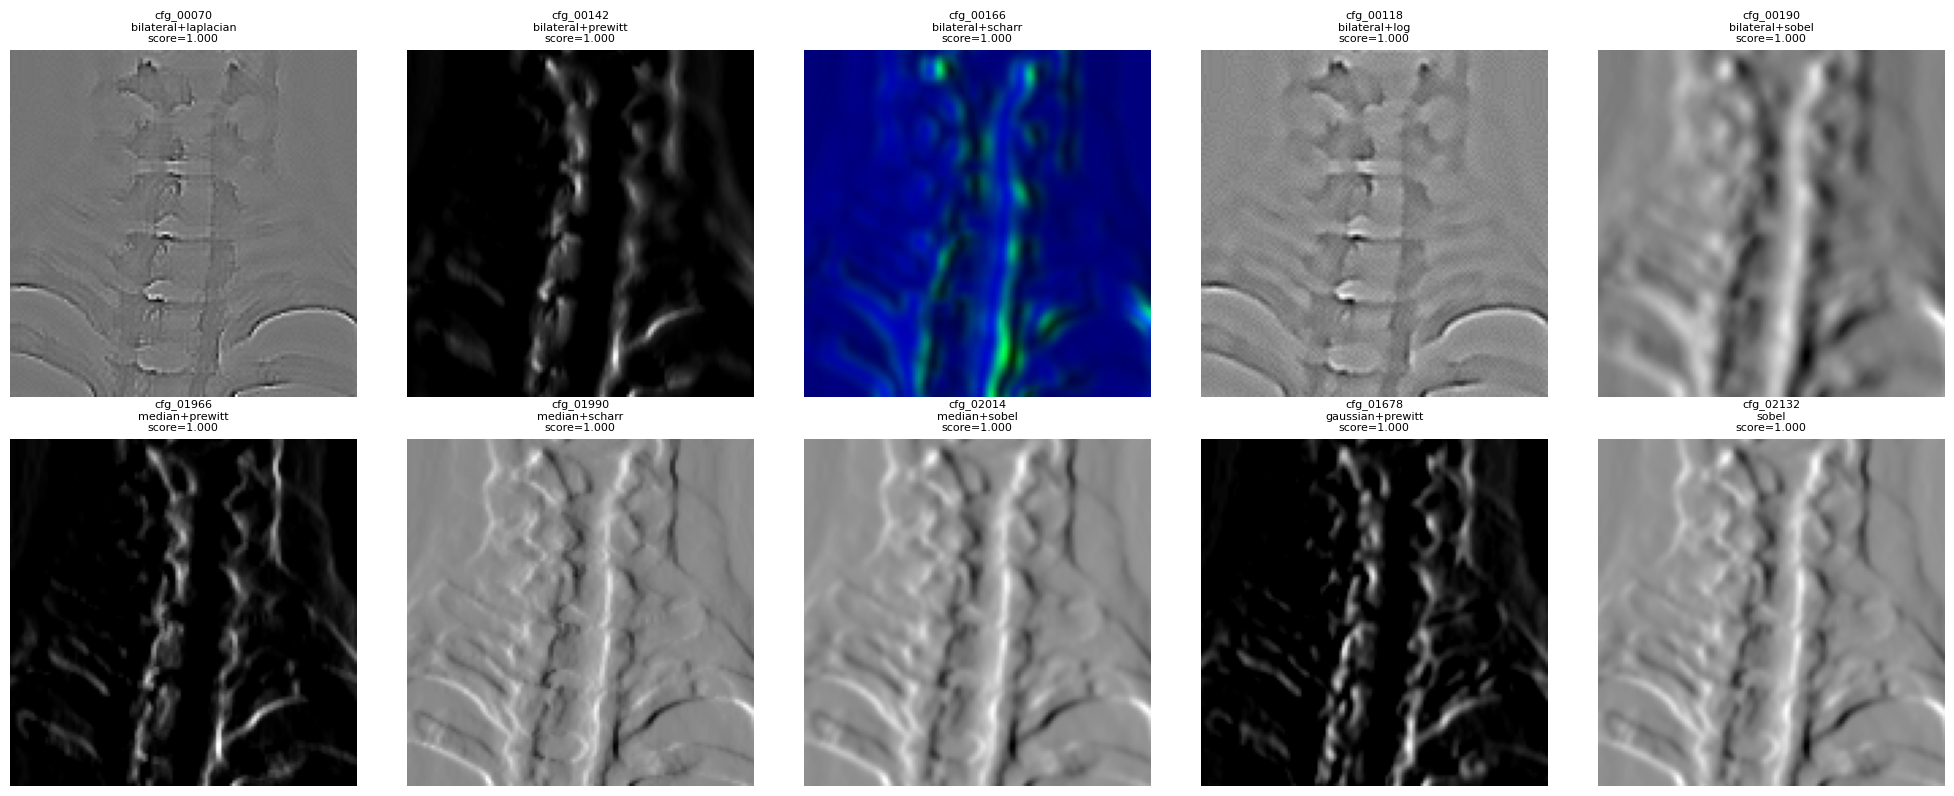
\includegraphics[width=\columnwidth]{images/Filtros.png}
\caption{
Comparación de filtros espaciales y operadores discretos de gradiente aplicados a radiografías de columna. Se evaluaron distintas combinaciones de filtros Gaussianos, bilaterales, Laplacianos, Sobel, Prewitt y Scharr con el objetivo de realzar estructuras anatómicas y mejorar las representaciones de entrada para la CNN.
}
\label{fig:filters}
\end{figure}

\begin{itemize}
    \item filtros pasa-bajas,
    \item filtros pasa-altas,
    \item filtros pasa-bandas,
    \item operadores discretos de gradiente,
    \item filtros basados en Fourier,
    \item operadores Sobel,
    \item operadores Prewitt,
    \item operadores Scharr,
    \item filtros Laplacianos,
    \item filtros Gaussianos,
    \item y filtros Bilaterales.
\end{itemize}

Los operadores de gradiente permitieron enfatizar discontinuidades locales y estructuras anatómicas relevantes, mientras que los filtros frecuenciales permitieron estudiar distintas componentes espaciales de la imagen.

Formalmente, una imagen radiográfica puede representarse mediante:

\[
I:\Omega \rightarrow \mathbb{R}
\]

y un filtro espacial discreto puede modelarse como una convolución:

\[
(I * K)(x,y)
=
\sum_{u}\sum_{v}
I(x-u,y-v)K(u,v)
\]

donde $K$ representa el kernel asociado al filtro utilizado.

En el caso de operadores discretos de gradiente, como Sobel o Prewitt, el objetivo consiste en aproximar derivadas espaciales de la imagen para detectar cambios abruptos de intensidad asociados a bordes anatómicos.

Todos estos filtros fueron evaluados mediante estudios de ablación con el objetivo de encontrar aquellas representaciones que aportaran una entrada más coherente y estructuralmente estable para la CNN.

Los resultados mostraron que ciertas combinaciones de filtros permitían preservar mejor la continuidad anatómica y mejorar la representación geométrica de la columna vertebral.


\begin{figure}[t]
\centering

\begin{minipage}{0.48\columnwidth}
\centering
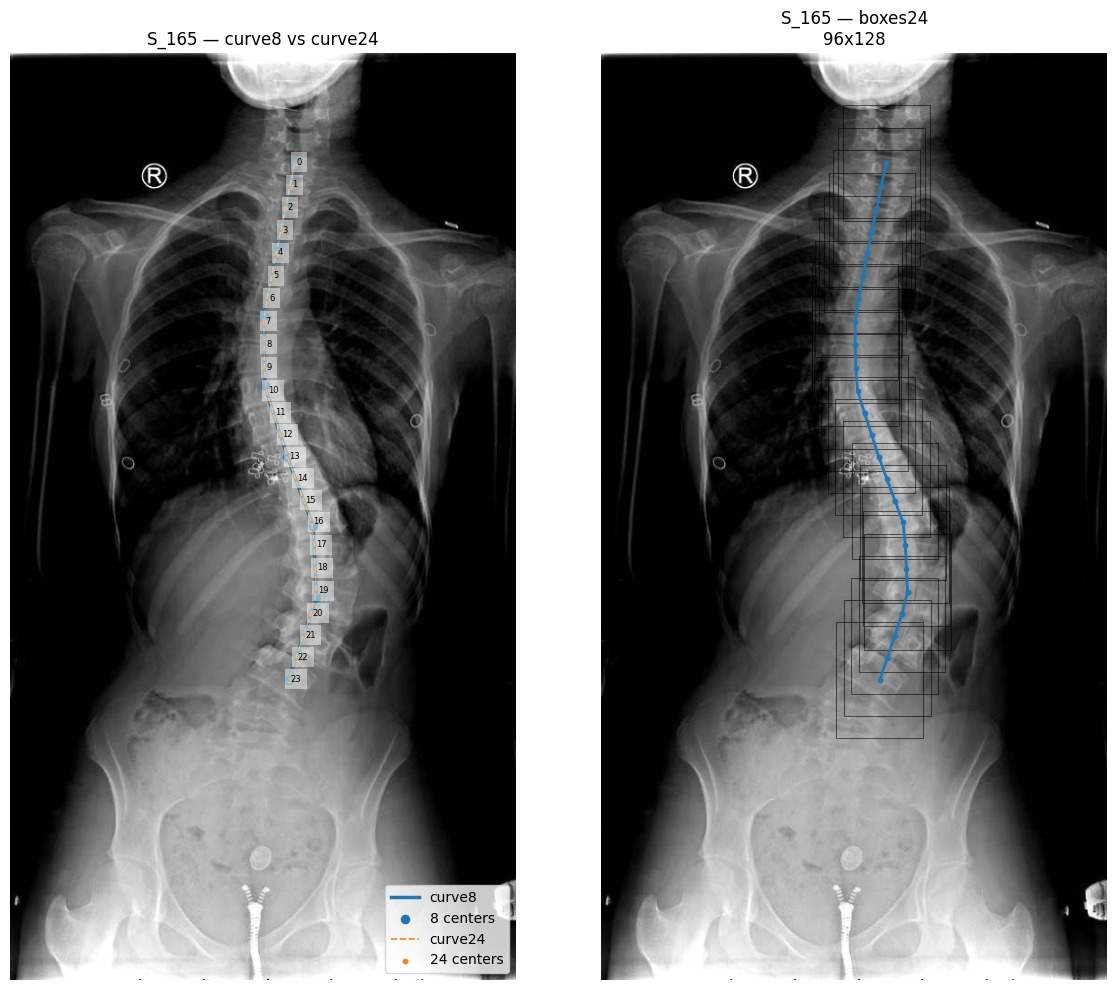
\includegraphics[width=\linewidth]{images/Parches1.jpeg}
\end{minipage}
\hfill
\begin{minipage}{0.48\columnwidth}
\centering
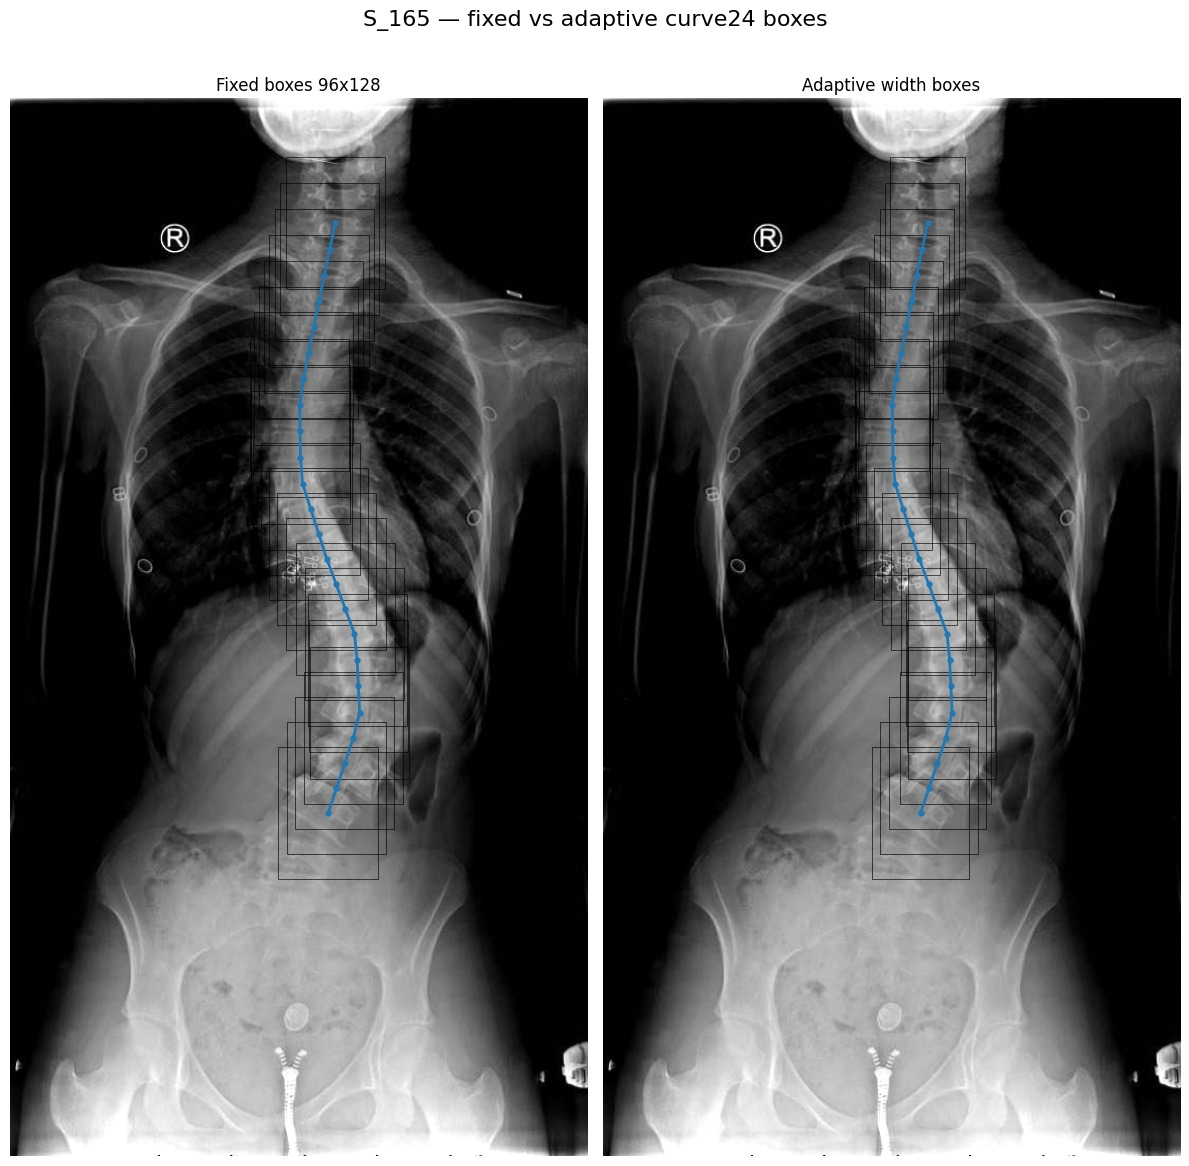
\includegraphics[width=\linewidth]{images/Parches2.jpeg}
\end{minipage}

\caption{
Construcción de parches anatómicos indexados sobre la curva vertebral. A partir de la trayectoria anatómica de la columna se generan vecindades locales discretas organizadas espacialmente sobre la curva. Se evaluaron estrategias de parches fijos y adaptativos para preservar continuidad anatómica y coherencia geométrica entre regiones consecutivas.
}
\label{fig:spine_patches}
\end{figure}

Después del análisis de filtros y representaciones espaciales, el siguiente paso consistió en modelar la columna vertebral mediante una representación anatómica ordenada basada en parches locales.

La columna fue aproximada mediante una curva central discreta obtenida a partir de centroides anatómicos distribuidos a lo largo de la estructura vertebral. A partir de esta curva se generó una familia indexada de vecindades locales:

\[
\{U_i\}_{i=1}^{N}
\]

donde cada $U_i$ representa un parche anatómico asociado a una región específica de la columna vertebral.

La indexación de los parches permite preservar continuidad espacial, relaciones de vecindad y orden anatómico entre regiones consecutivas. De esta manera, la columna puede interpretarse como una sucesión ordenada de subespacios discretos organizados sobre una trayectoria geométrica.


La \texttt{band\_mask} fue utilizada para restringir el análisis espacial a una vecindad anatómica local alrededor de la curva vertebral.

Esta representación define una región tubular discreta centrada sobre la trayectoria anatómica de la columna, permitiendo limitar el procesamiento únicamente a regiones estructuralmente relevantes.

La banda anatómica sirvió como restricción geométrica para:

\begin{itemize}
    \item reducir ruido estructural,
    \item preservar continuidad anatómica,
    \item mantener coherencia espacial,
    \item y proyectar representaciones derivadas de geometría diferencial sobre regiones anatómicamente relevantes.
\end{itemize}

Adicionalmente, la \texttt{band\_mask} permitió construir canales geométricos asociados a mapas de distancia, orientación local y representaciones tangenciales y normales alrededor de la columna vertebral.

\begin{figure}[t]
\centering
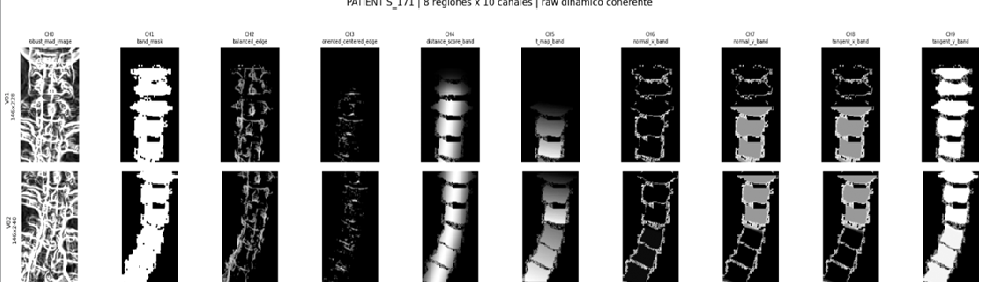
\includegraphics[width=\columnwidth]{images/ParcheCanales.png}
\caption{
Ejemplo de la representación geométrica multicanal generada a partir de parches de columna indexados anatómicamente. Cada canal codifica información estructural complementaria derivada de la curva anatómica y de la máscara vertebral binaria, incluyendo respuestas de borde, gradientes orientados, mapas de distancia y representaciones geométricas en banda. Estos canales proporcionan a la CNN contexto espacial y geométrico adicional más allá de la información de intensidad original.
}
\label{fig:geometric_channels}
\end{figure}

Adicionalmente, se evaluaron estrategias de parches de tamaño fijo y adaptativo, con el objetivo de preservar proporciones anatómicas y mantener coherencia estructural en distintas regiones de la columna vertebral.


\subsection{Parches anatómicos y organización estructural del dataset}

Una vez construido el espacio multicanal geométrico, la siguiente etapa consistió en dividir la columna vertebral en una secuencia ordenada de parches anatómicos locales.

El objetivo principal de esta estrategia fue enriquecer la representación espacial del dataset preservando simultáneamente:

\begin{itemize}
    \item continuidad anatómica,
    \item orden espacial,
    \item relaciones geométricas locales,
    \item y coherencia estructural entre regiones consecutivas de la columna vertebral.
\end{itemize}

Cada parche fue generado a partir de centroides distribuidos sobre la curva anatómica principal, respetando la progresión natural de la columna vertebral desde regiones superiores hacia regiones inferiores.

Formalmente, dada la curva anatómica:

\[
\gamma = \{c_i\}_{i=1}^{N}
\]

donde cada $c_i$ representa un centroide anatómico localizado sobre la trayectoria vertebral, se definió una familia ordenada de parches:

\[
\mathcal{U}=\{U_i\}_{i=1}^{N}
\]

donde cada subconjunto discreto $U_i$ corresponde a una vecindad anatómica local centrada alrededor del punto $c_i$.

La región anatómica completa se modeló como:

\[
\mathcal{CV}
=
\bigcup_{i=1}^{N} U_i
\]

preservando una estructura indexada sobre la curva vertebral.

Esta organización permitió que cada parche mantuviera una correspondencia anatómica consistente dentro del espacio de representación utilizado por la CNN.

Adicionalmente, cada parche fue enriquecido utilizando múltiples canales geométricos derivados de:

\begin{itemize}
    \item mapas de distancia,
    \item bandas anatómicas,
    \item gradientes orientados,
    \item vectores tangentes,
    \item vectores normales,
    \item y representaciones espaciales locales.
\end{itemize}

Esto permitió construir una representación estructuralmente enriquecida del espacio anatómico vertebral.

\subsection{Partición del dataset y validación}

Debido a que múltiples parches pertenecen a un mismo paciente, la validación del modelo debía evitar fugas de información anatómica entre conjuntos de entrenamiento y evaluación.

Por esta razón, la estrategia de validación cruzada (\textit{K-Fold Cross Validation}) fue realizada a nivel de paciente y no a nivel de parche.

Formalmente, sea:

\[
\mathcal{P}=\{p_1,p_2,\dots,p_M\}
\]

el conjunto de pacientes del dataset.

La partición se realizó sobre $\mathcal{P}$ de manera que todos los parches asociados a un mismo paciente permanecieran dentro del mismo subconjunto de entrenamiento, validación o prueba.

Esta restricción permitió:

\begin{itemize}
    \item evitar fuga de información,
    \item preservar independencia entre conjuntos,
    \item mantener coherencia anatómica,
    \item y obtener métricas de evaluación más realistas.
\end{itemize}

De esta manera, el modelo fue evaluado bajo un escenario clínicamente más consistente, donde las representaciones anatómicas de un paciente no aparecen simultáneamente en entrenamiento y prueba.



\subsection{CNN multicanal y utilización de targets anatómicos}

Con el objetivo de incorporar información geométrica y estructural adicional dentro del proceso de aprendizaje, se diseñó una CNN multicanal capaz de procesar simultáneamente distintas representaciones derivadas de la anatomía vertebral.

La entrada del modelo estuvo compuesta por un tensor multicanal de diez dimensiones espaciales, donde cada canal representa una señal específica asociada a la estructura de la columna vertebral.

Formalmente, la entrada puede expresarse como:

\[
X \in \mathbb{R}^{H \times W \times 10}
\]

donde $H$ y $W$ corresponden a las dimensiones espaciales del parche anatómico y los diez canales corresponden a distintas representaciones geométricas y espaciales.

Los canales utilizados fueron:

\begin{itemize}
    \item \texttt{robust\_mad\_image}
    \item \texttt{band\_mask}
    \item \texttt{balanced\_edge}
    \item \texttt{oriented\_centered\_edge}
    \item \texttt{distance\_score\_band}
    \item \texttt{t\_map\_band}
    \item \texttt{normal\_x\_band}
    \item \texttt{normal\_y\_band}
    \item \texttt{tangent\_x\_band}
    \item \texttt{tangent\_y\_band}
\end{itemize}

Cada uno de estos canales aporta información complementaria relacionada con:

\begin{itemize}
    \item intensidad radiográfica,
    \item continuidad anatómica,
    \item orientación espacial,
    \item geometría local,
    \item gradientes estructurales,
    \item y relaciones espaciales alrededor de la curva vertebral.
\end{itemize}

La hipótesis principal detrás de esta representación multicanal es que la CNN puede aprender no solamente patrones locales de intensidad, sino también relaciones geométricas asociadas a la anatomía de la columna vertebral.

\subsection{Targets anatómicos}

Para supervisar el entrenamiento de la red se utilizaron las anotaciones anatómicas del dataset, las cuales proporcionan información estructural a nivel de columna y vértebras.

Particularmente, el modelo fue entrenado utilizando:

\begin{itemize}
    \item máscaras binarias de la columna vertebral,
    \item segmentaciones multiclase de vértebras,
    \item representaciones de curva anatómica,
    \item y mapas espaciales derivados de las anotaciones originales.
\end{itemize}

Formalmente, el target de segmentación puede representarse como:

\[
Y:\Omega \rightarrow \{0,\dots,C-1\}
\]

donde cada píxel pertenece a una clase anatómica específica.

En el caso multiclase, cada vértebra fue representada mediante una etiqueta independiente, permitiendo que la CNN aprendiera separación anatómica entre regiones consecutivas.

Adicionalmente, las máscaras binarias fueron utilizadas para restringir espacialmente el aprendizaje y reforzar coherencia estructural dentro de la región vertebral.

La utilización simultánea de representaciones geométricas de entrada y targets anatómicos permitió construir una representación supervisada más consistente con la estructura real de la columna vertebral.





\subsection{Reconstrucción espacial de parches a partir de la salida de la CNN}

Una vez que los parches anatómicos enriquecidos fueron procesados por la CNN, las predicciones obtenidas no fueron interpretadas como regiones aisladas, sino como elementos de una representación espacial indexada de la columna vertebral.

Debido a que cada parche conserva su índice anatómico dentro de la curva vertebral, fue posible reconstruir nuevamente la organización espacial de la columna a partir de las salidas locales del modelo.

Formalmente, sea:

\[
\hat{Y}_i = f_\theta(U_i)
\]

la predicción de la CNN sobre el parche anatómico \(U_i\), donde \(i\) representa el índice asociado a la posición del parche sobre la curva vertebral.

La salida completa de la columna puede reconstruirse como una familia ordenada de predicciones:

\[
\hat{\mathcal{Y}} =
\{\hat{Y}_i\}_{i=1}^{N}
\]

preservando la relación de orden inducida por la curva:

\[
\hat{Y}_1 \leq \hat{Y}_2 \leq \cdots \leq \hat{Y}_N
\]

Esta organización permite mantener la coherencia anatómica de la columna vertebral después del procesamiento convolucional.

Desde una perspectiva topológica, cada predicción local puede interpretarse como una aproximación de un subespacio discreto asociado a una región anatómica. Por lo tanto, la reconstrucción global puede expresarse como:

\[
\hat{\mathcal{CV}}
=
\bigcup_{i=1}^{N} \hat{Y}_i
\]

donde \(\hat{\mathcal{CV}}\) representa la reconstrucción predicha de la región vertebral completa.

Esta formulación permite conservar información espacial y topológica durante el flujo del modelo, ya que las predicciones locales mantienen su pertenencia a una familia indexada de subespacios discretos.

En consecuencia, la CNN no solamente produce máscaras locales, sino una representación anatómica reconstruible, ordenada e indexada, compatible con la estructura geométrica original de la columna vertebral.

La conservación del orden anatómico permite:

\begin{itemize}
    \item reubicar cada parche en su posición espacial correspondiente,
    \item evitar saltos entre regiones vertebrales consecutivas,
    \item preservar continuidad estructural,
    \item mantener correspondencia entre curva, parche y predicción,
    \item y reconstruir una representación global de la columna a partir de salidas locales.
\end{itemize}

De esta manera, el modelo aprovecha una propiedad topológica fundamental: la columna puede analizarse como una unión ordenada de subespacios discretos, donde cada subespacio conserva relaciones de vecindad y pertenencia dentro de la estructura anatómica completa.


\begin{figure}[t]
\centering
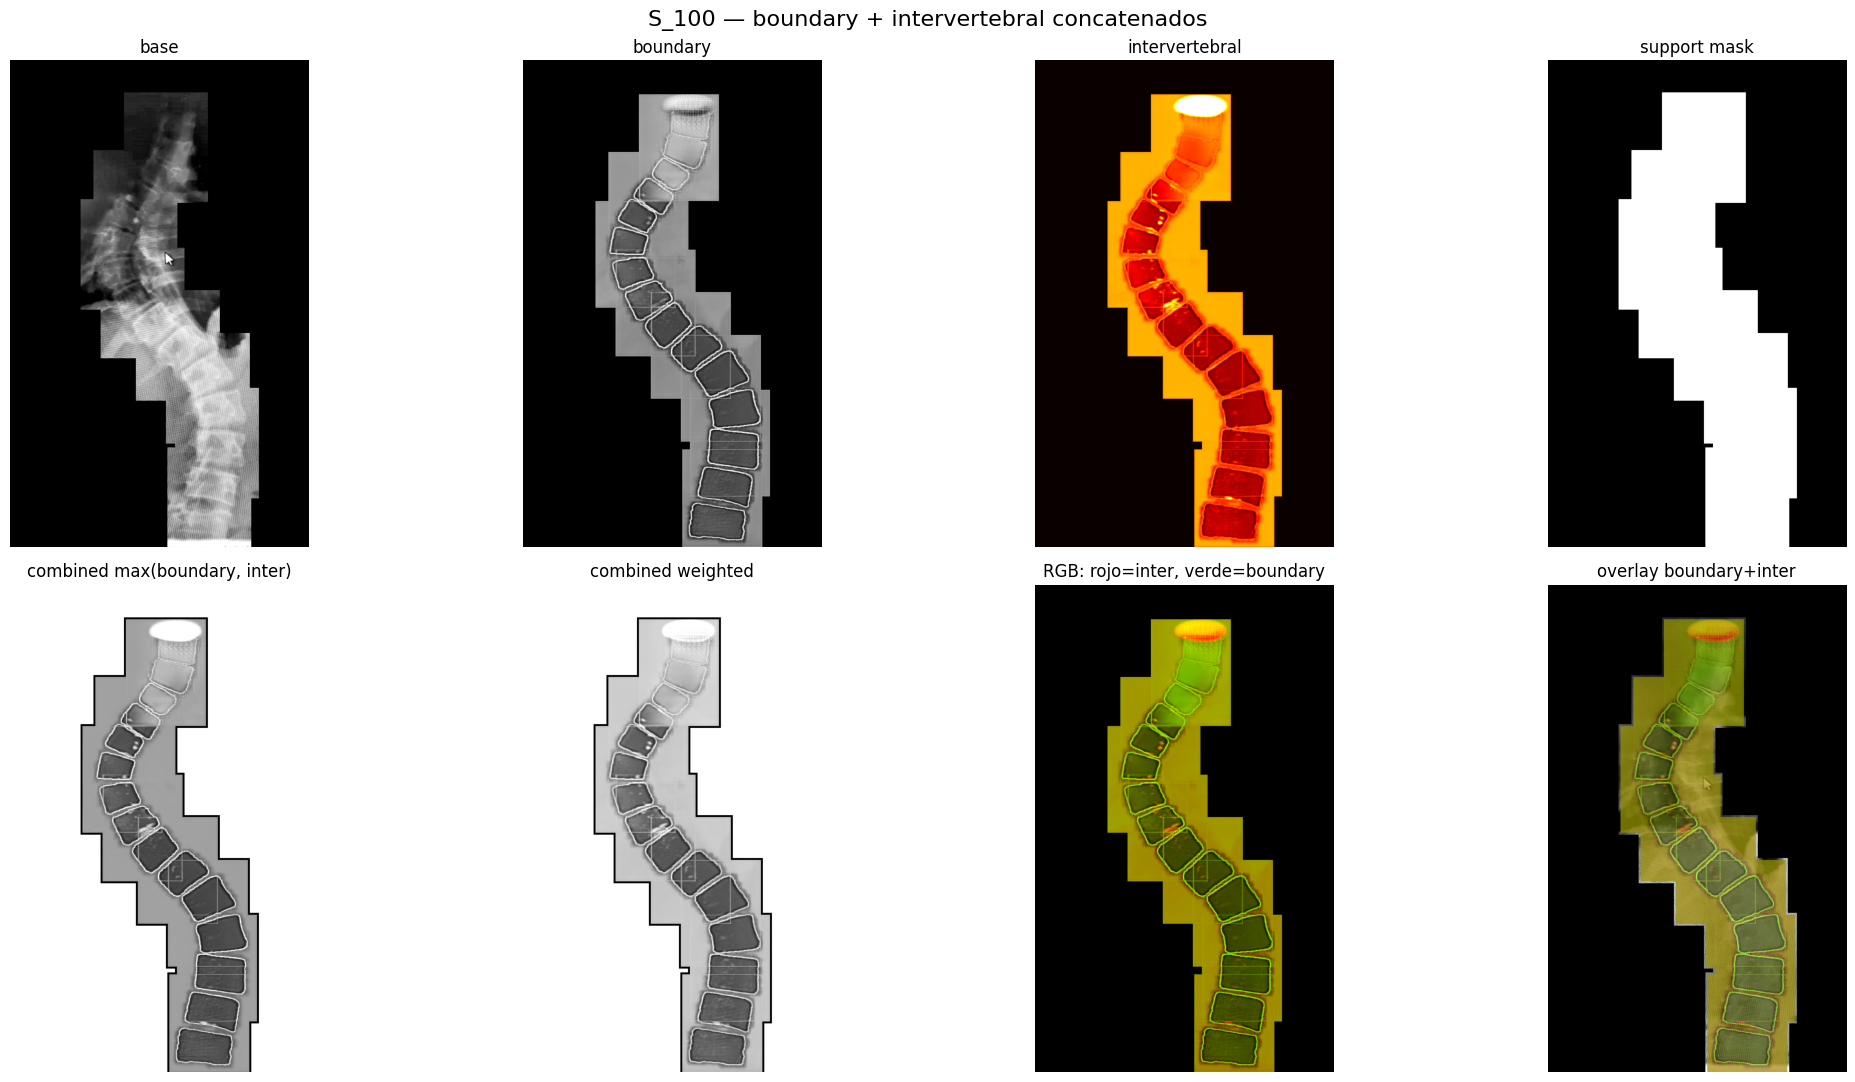
\includegraphics[width=\columnwidth]{images/Reconstruccion.png}
\caption{
Reconstrucción espacial de parches vertebrales indexados después del procesamiento por la CNN. Las predicciones locales de bordes e información intervertebral son reorganizadas respetando el orden anatómico sobre la curva vertebral, permitiendo reconstruir una representación global coherente de la columna vertebral y preservando continuidad anatómica y relaciones espaciales locales.
}
\label{fig:spatial_reconstruction}
\end{figure}


\subsection{Análisis frecuencial de gaps y picos anatómicos}

Con el objetivo de mejorar la separación entre regiones vertebrales y proporcionar mayor contexto anatómico al modelo, se realizó un análisis frecuencial sobre las representaciones reconstruidas de la columna vertebral.

La hipótesis principal fue que las transiciones anatómicas entre vértebras generan patrones estructurales característicos en el dominio frecuencial, particularmente asociados a:

\begin{itemize}
    \item picos de intensidad,
    \item discontinuidades locales,
    \item regiones intervertebrales,
    \item y gaps anatómicos entre vértebras consecutivas.
\end{itemize}

A partir de las representaciones reconstruidas por la CNN, se analizaron perfiles espaciales y frecuenciales para detectar cambios estructurales asociados a separaciones vertebrales.

Formalmente, dada una representación espacial reconstruida:

\[
R:\Omega \rightarrow \mathbb{R}
\]

se calculó una representación frecuencial:

\[
\mathcal{F}(R)
\]

permitiendo estudiar componentes de alta y baja frecuencia asociadas a cambios anatómicos locales.

Los picos frecuenciales obtenidos permitieron identificar regiones con alta variación estructural, mientras que los gaps representaron posibles zonas intervertebrales y separaciones anatómicas entre vértebras consecutivas.

Posteriormente, estas señales frecuenciales fueron intersectadas con la curva anatómica principal:

\[
\gamma = \{c_i\}_{i=1}^{N}
\]

con el objetivo de preservar correspondencia espacial respecto a la organización vertebral original.

Formalmente, la representación contextual final puede expresarse como:

\[
\mathcal{S}
=
\mathcal{F}(R)
\cap
\gamma
\]

donde:

\begin{itemize}
    \item $\mathcal{F}(R)$ representa la señal frecuencial reconstruida,
    \item $\gamma$ representa la curva anatómica vertebral,
    \item y $\mathcal{S}$ corresponde a una representación frecuencial anatómicamente restringida.
\end{itemize}

Esta intersección permitió asociar patrones frecuenciales locales con regiones anatómicas específicas de la columna vertebral, proporcionando contexto espacial adicional al modelo.

Como resultado, las señales frecuenciales no solamente representaron cambios de intensidad, sino también transiciones anatómicas relevantes entre vértebras consecutivas, ayudando a preservar coherencia estructural durante la segmentación.


\begin{figure}[t]
\centering
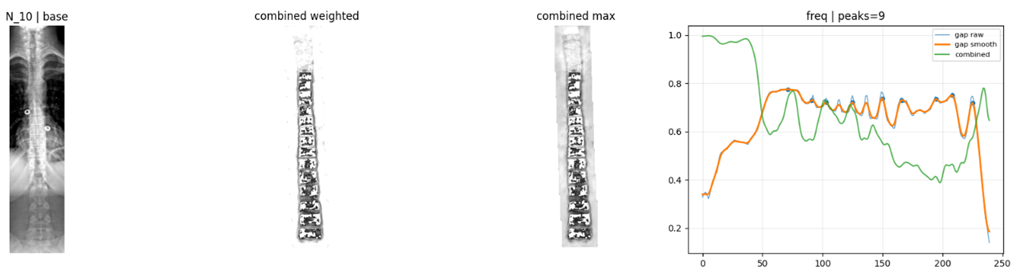
\includegraphics[width=\columnwidth]{images/Ferecuencua.png}
\caption{
Análisis frecuencial aplicado sobre representaciones reconstruidas de la columna vertebral. La figura muestra la combinación de mapas estructurales y el análisis de picos y gaps frecuenciales asociados a regiones intervertebrales. La intersección entre la señal frecuencial y la curva anatómica permitió preservar correspondencia espacial y proporcionar mayor contexto anatómico durante la segmentación.
}
\label{fig:frequency_analysis}
\end{figure}


\subsection{Clusterización de representaciones anatómicas}

Después de reconstruir las representaciones espaciales y analizar las señales frecuenciales asociadas a gaps y picos intervertebrales, se realizó una etapa de clusterización con el objetivo de estudiar la organización latente de las muestras.

La finalidad de esta etapa fue analizar si las representaciones obtenidas conservaban información anatómica suficiente para agrupar pacientes o regiones con patrones estructurales similares.

Para ello, cada paciente o región anatómica fue representado mediante un vector de características:

\[
z_i \in \mathbb{R}^{d}
\]

donde \(z_i\) contiene información derivada de:

\begin{itemize}
    \item representaciones CNN,
    \item señales geométricas,
    \item mapas intervertebrales,
    \item señales frecuenciales,
    \item y descriptores topológicos.
\end{itemize}

El conjunto completo de representaciones se definió como:

\[
Z = \{z_1,z_2,\dots,z_n\}
\]

Posteriormente, se aplicaron técnicas de reducción dimensional y clusterización para visualizar la estructura del espacio latente:

\[
\phi: \mathbb{R}^{d} \rightarrow \mathbb{R}^{2}
\]

donde \(\phi\) representa una proyección de baja dimensión, como PCA o UMAP.

Sobre este espacio proyectado se evaluaron agrupamientos con el objetivo de identificar separabilidad entre configuraciones anatómicas.

La clusterización permitió estudiar:

\begin{itemize}
    \item separación entre patrones normales y escolióticos,
    \item agrupamientos asociados a variaciones morfológicas,
    \item consistencia de las representaciones geométricas,
    \item y estabilidad del espacio latente generado por el modelo.
\end{itemize}

Esta etapa no se utilizó como mecanismo principal de segmentación, sino como una herramienta de análisis para evaluar si las representaciones aprendidas capturaban estructura anatómica relevante.

\subsection{Modelo estudiante para generación de curva y perfil geométrico}

Posteriormente, se planteó un modelo estudiante orientado a reducir la complejidad computacional del pipeline y generar una representación geométrica más compacta de la columna vertebral.

A diferencia del modelo multicanal, el estudiante recibe una entrada de menor dimensionalidad y aprende a aproximar salidas estructurales derivadas del modelo principal, tales como la máscara vertebral, la curva anatómica y el perfil geométrico asociado.

Formalmente, sea:

\[
X_s \in \mathbb{R}^{H \times W \times c_s}
\]

la entrada del modelo estudiante, donde \(c_s < 10\) representa un número reducido de canales.

El objetivo del estudiante es aprender una función:

\[
f_s:X_s \rightarrow (\hat{M}, \hat{\gamma}, \hat{G})
\]

donde:

\begin{itemize}
    \item \(\hat{M}\) representa la máscara vertebral estimada,
    \item \(\hat{\gamma}\) representa la curva anatómica predicha,
    \item \(\hat{G}\) representa el perfil geométrico de la columna.
\end{itemize}

El perfil geométrico \(\hat{G}\) puede incluir información derivada de:

\begin{itemize}
    \item orientación local,
    \item curvatura aproximada,
    \item continuidad anatómica,
    \item mapas de distancia,
    \item tangentes,
    \item normales,
    \item y regiones intervertebrales.
\end{itemize}

De esta manera, el modelo estudiante no busca únicamente segmentar píxeles, sino aprender una representación estructural compacta capaz de describir la geometría global de la columna vertebral.

La curva anatómica generada por el estudiante se puede expresar como una sucesión ordenada de puntos:

\[
\hat{\gamma}=\{\hat{c}_i\}_{i=1}^{N}
\]

donde cada \(\hat{c}_i\) corresponde a un centroide predicho sobre la trayectoria vertebral.

A partir de esta curva se pueden reconstruir nuevamente regiones locales, parches anatómicos o bandas tubulares, preservando el orden espacial de la columna:

\[
\hat{\mathcal{CV}}
=
\bigcup_{i=1}^{N} \hat{U}_i
\]

donde cada \(\hat{U}_i\) representa una vecindad local generada alrededor del centroide predicho \(\hat{c}_i\).

Este enfoque permite utilizar el modelo estudiante como una etapa ligera de inferencia, capaz de producir una aproximación anatómica inicial que posteriormente puede ser utilizada para:

\begin{itemize}
    \item reconstruir la curva vertebral,
    \item generar perfiles geométricos,
    \item reducir el costo computacional,
    \item apoyar la segmentación final,
    \item y facilitar análisis posteriores como TDA, clustering o estimación del ángulo de Cobb.
\end{itemize}

En este sentido, el modelo estudiante funciona como una aproximación eficiente del conocimiento geométrico aprendido por el pipeline completo, manteniendo la información estructural más relevante para el análisis anatómico.

\subsection{Infraestructura experimental y despliegue}

La infraestructura experimental utilizada para el entrenamiento y despliegue del pipeline fue diseñada bajo una arquitectura distribuida orientada a microservicios y procesamiento escalable.

El sistema fue desarrollado principalmente utilizando Python debido a su integración con bibliotecas de aprendizaje profundo, procesamiento de imágenes médicas y análisis científico.

Para la ejecución de contenedores y despliegue de servicios se utilizaron tecnologías basadas en Docker y Amazon ECS (\textit{Elastic Container Service}), permitiendo escalar distintos componentes del pipeline de manera independiente.

La infraestructura cloud fue administrada mediante Terraform, permitiendo definir recursos de infraestructura como código (\textit{Infrastructure as Code, IaC}) y facilitando reproducibilidad y automatización del entorno experimental.

Adicionalmente, se utilizaron servicios de almacenamiento en memoria utilizando Redis para:

\begin{itemize}
    \item almacenamiento temporal de resultados,
    \item manejo de caché,
    \item sincronización de procesos,
    \item y optimización de acceso a representaciones intermedias.
\end{itemize}

Para el procesamiento distribuido y la ejecución de cargas experimentales se evaluaron entornos orquestados mediante Kubernetes y Elastic Kubernetes Service (EKS), permitiendo ejecutar experimentos paralelos asociados a:

\begin{itemize}
    \item entrenamiento CNN,
    \item generación de canales geométricos,
    \item reconstrucción espacial,
    \item análisis TDA,
    \item y clusterización.
\end{itemize}

La arquitectura general permitió desacoplar distintas etapas del pipeline, facilitando escalabilidad, modularidad y distribución de recursos computacionales.

Finalmente, la infraestructura experimental fue diseñada para soportar entrenamiento sobre GPU, procesamiento paralelo y almacenamiento persistente de artefactos experimentales, incluyendo:

\begin{itemize}
    \item modelos entrenados,
    \item representaciones anatómicas,
    \item embeddings topológicos,
    \item métricas experimentales,
    \item y reconstrucciones espaciales.
\end{itemize}


\begin{figure}[t]
\centering
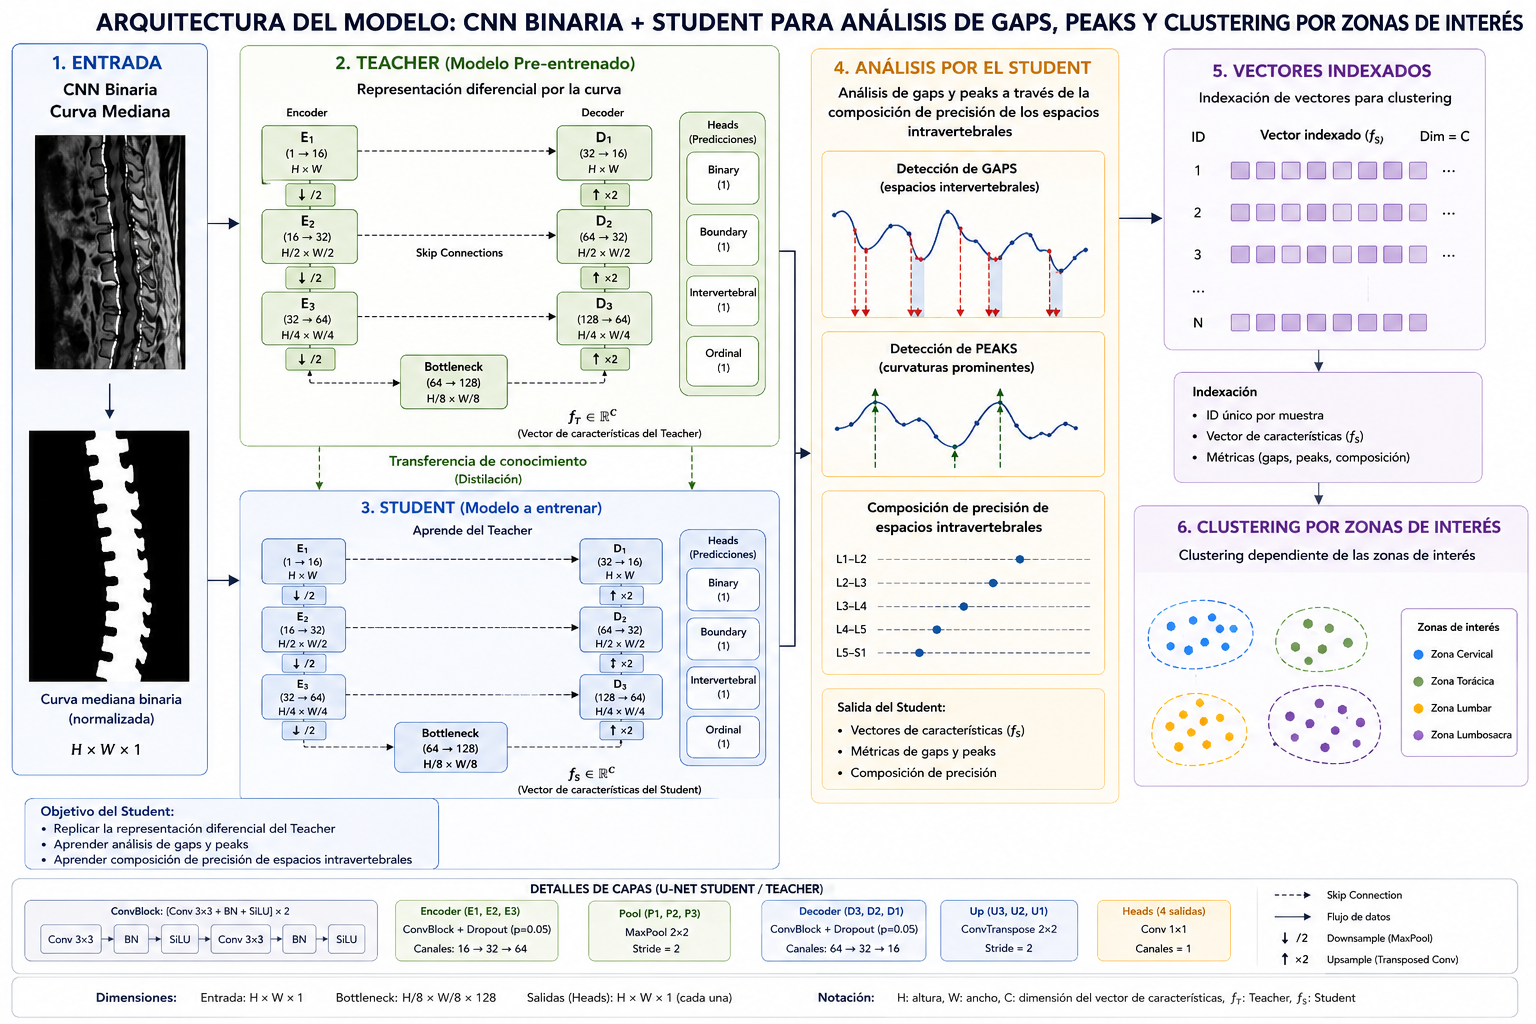
\includegraphics[width=\columnwidth]{images/Diagrama.png}
\caption{
Arquitectura general del pipeline propuesto. El modelo combina una CNN binaria, un modelo teacher--student y análisis geométrico basado en gaps y picos intervertebrales. Las representaciones generadas son reorganizadas mediante indexación anatómica para construir vectores estructurales utilizados posteriormente en procesos de clustering por zonas de interés anatómico.
}
\label{fig:teacher_student_pipeline}
\end{figure}

\subsection{Visión General}

La metodología propuesta combina representaciones anatómicas, geométricas y topológicas con modelos de aprendizaje profundo para construir una representación estructuralmente enriquecida de la columna vertebral.

El flujo general del modelo inicia con el preprocesamiento y normalización de radiografías vertebrales, seguido por la construcción de una curva anatómica central utilizada para generar regiones tubulares y parches anatómicos indexados.

Posteriormente, se construye un espacio multicanal utilizando representaciones geométricas derivadas de la curva vertebral, incluyendo mapas de distancia, gradientes orientados, máscaras anatómicas y representaciones tangenciales y normales.

Estas representaciones son procesadas mediante una CNN multicanal encargada de aprender patrones anatómicos locales y relaciones espaciales entre vértebras consecutivas.

A diferencia de enfoques convencionales basados únicamente en intensidad radiográfica, el modelo propuesto incorpora restricciones geométricas y organización anatómica explícita dentro del proceso de aprendizaje.

Finalmente, las salidas locales generadas por la CNN son reorganizadas utilizando la indexación anatómica definida sobre la curva vertebral, permitiendo reconstruir una representación global coherente de la columna vertebral.



\subsection{Dataset}

El dataset utilizado contiene radiografías anteroposteriores de columna vertebral
correspondientes a pacientes con y sin escoliosis. Cada imagen incluye diferentes
niveles de anotación que permiten analizar la estructura anatómica de la columna.

Las representaciones disponibles incluyen:

\begin{itemize}

\item \textbf{Radiografía original}: imagen médica en escala de grises.

\item \textbf{Máscara binaria}: segmentación de la columna vertebral donde los
píxeles pertenecientes a la columna toman valor 255 y el resto corresponde al fondo.

\item \textbf{Segmentación multiclase}: cada vértebra se representa con una etiqueta
independiente (por ejemplo C7, T1--T12, L1--L5).

\item \textbf{Curva espinal}: línea central de la columna estimada a partir de la
máscara segmentada.

\item \textbf{Métricas clínicas}: cálculo automático del ángulo de Cobb,
utilizado para cuantificar la severidad de la escoliosis.

\end{itemize}





A partir de la segmentación es posible obtener representaciones geométricas
de la columna vertebral. En particular, se puede estimar la línea central
de la columna y calcular métricas clínicas como el ángulo de Cobb, ampliamente
utilizado en la práctica médica para evaluar la severidad de la escoliosis.






\label{fig:eda_dataset_profile}

\end{figure}

```latex

\subsection{Evaluación cualitativa y cuantitativa de la CNN}

La CNN fue entrenada sobre parches anatómicos derivados de la curva espinal. 
Cada parche contiene canales de entrada estructurales, incluyendo la imagen normalizada, 
la banda anatómica, bordes y respuestas orientadas. A partir de estos canales, el modelo 
produce varias salidas: segmentación multiclase regional, máscara binaria, bordes, espacios 
intervertebrales y mapa ordinal.

\begin{figure}[H]
\centering
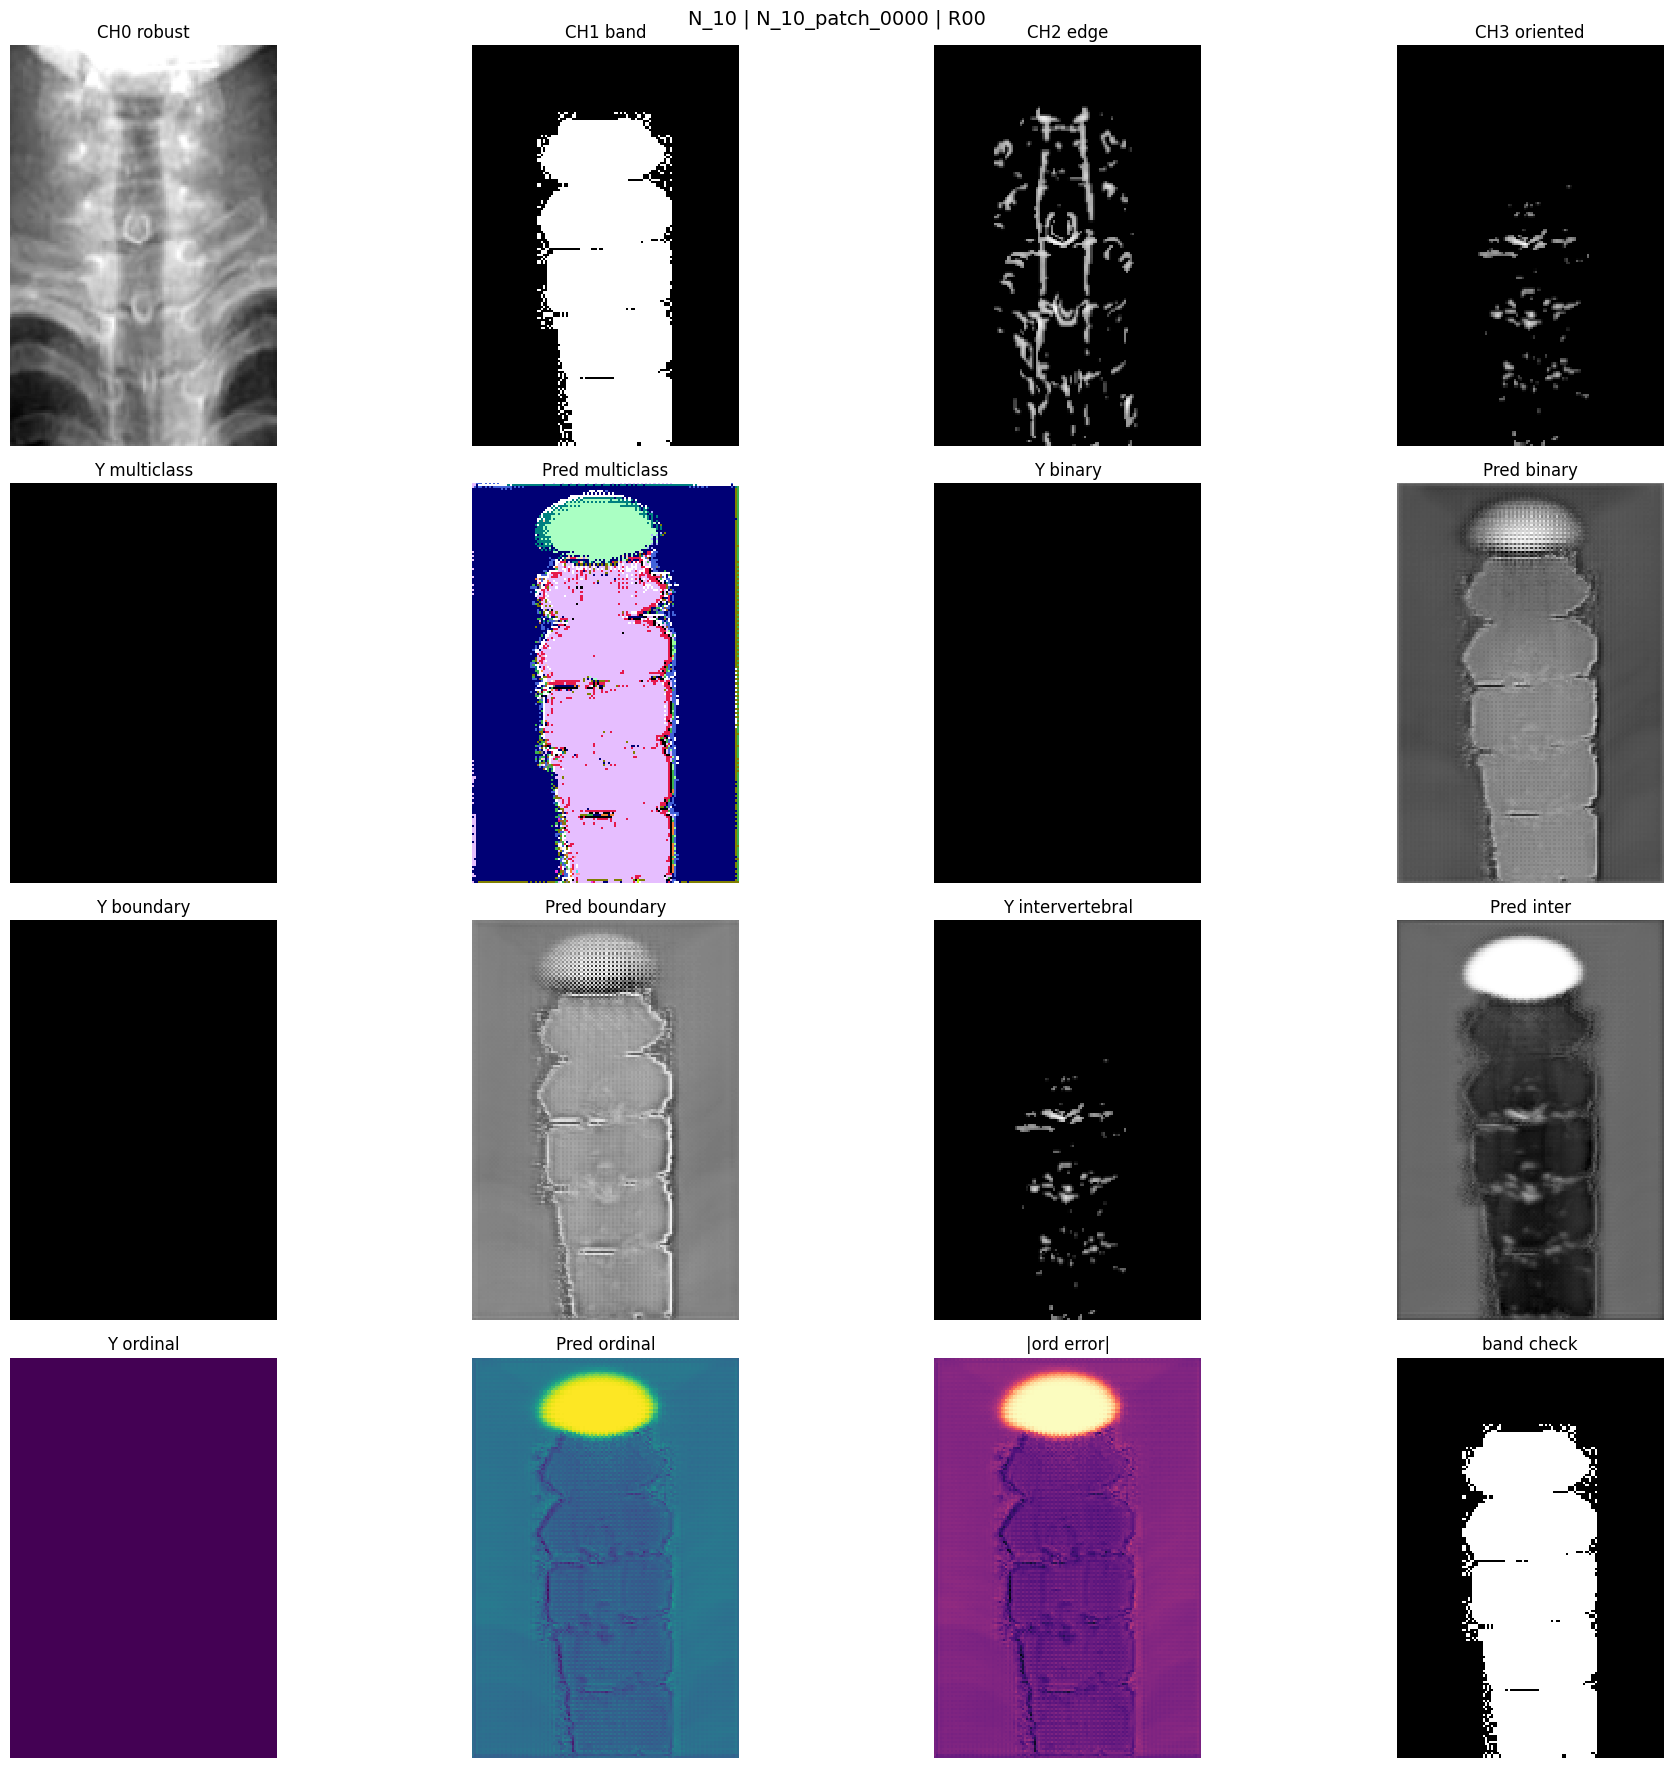
\includegraphics[width=0.40\textwidth]{images/preidconCNN.png}
\caption{
Ejemplo de predicción multisalida de la CNN sobre un parche anatómico de la columna. 
La parte superior muestra los canales de entrada utilizados por el modelo: imagen robustamente 
normalizada, máscara de banda, mapa de bordes y respuesta orientada. Las salidas muestran la 
comparación entre las máscaras objetivo y las predicciones para segmentación multiclase, máscara 
binaria, bordes, espacios intervertebrales y mapa ordinal. Esta visualización permite comprobar 
que la CNN aprende una representación estructural de la región vertebral, integrando información 
de intensidad, borde y geometría local.
}
\label{fig:cnn_multihead_prediction}
\end{figure}}



Estos resultados muestran que la CNN aprende de manera temprana la estructura binaria de la 
columna, ya que la métrica binaria alcanza valores altos desde las primeras épocas. Sin embargo, 
la segmentación regional multiclase presenta mayor dificultad, reflejada en valores bajos de Dice. 
Esto es esperable porque la tarea regional exige distinguir límites anatómicos finos entre vértebras 
y espacios intervertebrales. Por lo tanto, la CNN funciona adecuadamente como extractor geométrico 
inicial, pero requiere estrategias adicionales de refinamiento para mejorar la separación regional.


\subsection{Evidencia de la clusterización regional}


La clusterización regional se realizó sobre vectores anatómicamente indexados derivados de la curva espinal estimada por la CNN. Cada fila del archivo \texttt{region\_3d\_coordinates\_for\_report.csv} representa una región anatómica asociada a una vértebra y a un paciente. Estas regiones conservan información clínica, geométrica y morfológica, incluyendo la clase del paciente, el identificador vertebral, la zona de la curva, el tipo de afectación regional, el cluster asignado, la probabilidad máxima de asignación, la distancia al ápice, la distancia al eje CSVL, la altura del pico, la fuerza del gap intervertebral y las longitudes de onda vecinas.

El análisis no se realizó sobre la imagen completa, sino sobre regiones anatómicas ordenadas a lo largo de la curva espinal. Esto permite interpretar cada cluster como un tipo de patrón regional vertebral o paravertebral, asociado con características geométricas similares.

\subsubsection{Evidencias cuantitativas}

El conjunto de datos regional contiene 2210 regiones descritas por 88 variables, además de una tabla de probabilidades de cluster y un resumen de 24 clusters. Esto indica que el análisis fue realizado sobre una representación regional amplia, no sobre ejemplos aislados.

La comparación de modelos de clusterización mostró que la mejor configuración fue la representación \texttt{robust\_kpca\_poly} combinada con el modelo \texttt{gmm\_tied}. Esta configuración obtuvo los siguientes resultados:

\begin{table}[H]
\centering
\caption{Mejor configuración de clusterización regional.}
\label{tab:best_clustering_model}
\begin{tabular}{lc}
\hline
\textbf{Métrica} & \textbf{Valor} \\
\hline
Representación & \texttt{robust\_kpca\_poly} \\
Modelo & \texttt{gmm\_tied} \\
Clusters solicitados & 24 \\
Clusters encontrados & 24 \\
Silhouette & 0.261442 \\
Davies--Bouldin & 1.121589 \\
Calinski--Harabasz & 193.519791 \\
Pureza dominante media & 0.829408 \\
Tasa media de escoliosis & 0.792215 \\
Quality score & 0.484308 \\
\hline
\end{tabular}
\end{table}

Estos resultados sugieren que la combinación de normalización robusta, Kernel PCA polinomial y un modelo de mezcla gaussiana con covarianza compartida permitió obtener una separación útil entre tipos regionales. Aunque el valor de \textit{silhouette} no indica una separación perfecta, la pureza dominante media muestra que los clusters tienden a estar dominados por una clase principal.

\subsubsection{Clusters asociados con escoliosis}

Una evidencia importante es que algunos clusters estuvieron compuestos exclusivamente por regiones provenientes de pacientes con escoliosis. En particular, los clusters 3, 21, 10, 18 y 15 presentaron una tasa de escoliosis igual a 1.0 y una pureza dominante igual a 1.0.

\begin{table}[H]
\centering
\caption{Clusters regionales dominados completamente por escoliosis.}
\label{tab:scoliosis_dominant_clusters}
\begin{tabular}{ccccc}
\hline
\textbf{Cluster} & \textbf{Regiones} & \textbf{Pacientes} & \textbf{Tasa de escoliosis} & \textbf{Pureza dominante} \\
\hline
3  & 17 & 2  & 1.0 & 1.0 \\
21 & 14 & 12 & 1.0 & 1.0 \\
10 & 11 & 11 & 1.0 & 1.0 \\
18 & 8  & 7  & 1.0 & 1.0 \\
15 & 1  & 1  & 1.0 & 1.0 \\
\hline
\end{tabular}
\end{table}

Estos clusters representan zonas regionales cuya geometría, posición anatómica y comportamiento morfológico se asociaron exclusivamente con pacientes escolióticos dentro del conjunto analizado. Por esta razón, pueden interpretarse como regiones de interés para el análisis posterior con TDA y para la caracterización local de la deformidad espinal.

\subsubsection{Interpretación}

Los resultados indican que la curva reconstruida por la CNN permitió transformar cada radiografía en una secuencia anatómica regional. A partir de esta curva se obtuvieron variables como la posición normalizada sobre la trayectoria, la distancia al ápice, la distancia al eje CSVL, la altura de los picos y la fuerza de los gaps intervertebrales. Estas variables generaron un espacio de características donde las regiones con morfología similar quedaron próximas entre sí.

La presencia de clusters con pureza escoliótica del 100\% sugiere que el modelo no solamente segmenta la estructura de la columna, sino que también produce descriptores regionales útiles para identificar zonas de afectación. En este sentido, la segmentación de la curva funciona como una etapa de extracción geométrica, mientras que la clusterización funciona como una etapa de descubrimiento de patrones anatómicos regionales.

\subsubsection{Conclusión}

La evidencia obtenida demuestra que la representación regional derivada de la CNN conserva información anatómica relevante para diferenciar patrones normales y escolióticos. La mejor configuración, basada en \texttt{robust\_kpca\_poly} y \texttt{gmm\_tied}, logró formar 24 clusters con una pureza dominante media de 0.8294. Además, varios clusters mostraron una composición completamente escoliótica, lo cual respalda la utilidad del enfoque para detectar regiones de interés asociadas con deformidad espinal.

Por lo tanto, la segmentación de la curva no debe interpretarse únicamente como una salida visual, sino como una representación geométrica estructurada que permite construir perfiles regionales, analizar la distribución de afectación y preparar vectores anatómicos para etapas posteriores de TDA, reducción dimensional y clasificación.
```

\section{Trabajo Futuro}

Como trabajo futuro se plantea extender el modelo a datasets clínicos más grandes, explorar representaciones topológicas más avanzadas y evaluar el modelo en escenarios clínicos reales.

También se investigará la incorporación de modelos generativos y aprendizaje auto-supervisado para mejorar la generalización en entornos con datos limitados.
\nocite{*}
\bibliographystyle{IEEEtran}
\bibliography{referencias}

\begin{thebibliography}{99}

\bibitem{hu2019topology}
X. Hu, F. Li, D. Samaras, and C. Chen, 
``Topology-Preserving Deep Image Segmentation,'' 
\emph{arXiv preprint arXiv:1906.05404}, 2019.

\bibitem{clough2019topological}
J. R. Clough, N. Byrne, I. Oksuz, V. A. Zimmer, J. A. Schnabel, and A. P. King, 
``A Topological Loss Function for Deep-Learning Based Image Segmentation Using Persistent Homology,'' 
\emph{IEEE Transactions on Pattern Analysis and Machine Intelligence}, 2019.

\bibitem{hu2021morse}
X. Hu, Y. Wang, F. Li, D. Samaras, and C. Chen, 
``Topology-Aware Segmentation Using Discrete Morse Theory,'' 
\emph{arXiv preprint arXiv:2103.09992}, 2021.

\bibitem{everat1996topological}
J.-C. Everat and G. Bertrand, 
``New Topological Operators for Segmentation,'' 
in \emph{Proceedings of the 3rd IEEE International Conference on Image Processing}, 1996.

\bibitem{lux2024topograph}
L. Lux, J. Paetzold, and collaborators, 
``Topograph: An Efficient Graph-Based Framework for Strictly Topology Preserving Image Segmentation,'' 
\emph{arXiv preprint}, 2024.

\end{thebibliography}

\end{document}